\documentclass[11pt,a4paper]{article}
\usepackage[margin=20mm,headheight=16pt]{geometry}
\usepackage{fontspec,kotex,amsmath,booktabs,longtable,array,xcolor,hyperref,fancyhdr,graphicx}
\setmainfont{DejaVu Serif}
\setsansfont{DejaVu Sans}
\setmonofont{DejaVu Sans Mono}
\setmainhangulfont{Noto Sans CJK KR}
\setmonohangulfont{Noto Sans CJK KR}
\definecolor{navy}{HTML}{173E59}
\definecolor{codebg}{HTML}{F3F6F8}
\hypersetup{colorlinks=true,linkcolor=navy,urlcolor=navy,pdftitle={GuardSynth Experimental Evaluation}}
\urlstyle{same}
\setlength{\parindent}{0pt}
\setlength{\parskip}{4pt}
\setlength{\emergencystretch}{4em}
\setlength{\tabcolsep}{4pt}
\renewcommand{\arraystretch}{1.2}
\pagestyle{fancy}\fancyhf{}
\fancyhead[L]{\small GuardSynth}
\fancyhead[R]{\small Experimental Evaluation}
\fancyfoot[C]{\thepage}
\renewcommand{\headrulewidth}{0.3pt}
\clubpenalty=10000\widowpenalty=10000
\raggedbottom
\begin{document}

\section*{실험 및 결과}

\section*{A. 평가 목적과 설정}

본 실험은 명시적 행동 제약을 CoC에 더했을 때의 행동 선택 효과와, 그 제약을 EBLC로 명세·검증하여 CNL로 제공하는 개발 경로의 검사 가능성을 구분하여 평가한다. P1과 P2는 모두 우리의 제약 강화 접근이다. P1–P2 비교는 경쟁 기법 간 우열이 아니라 정형화된 지원 경로에서도 행동 효과가 유지되는지 살펴보는 보조 비교이다.\par

\par\smallskip\noindent\begin{minipage}{\linewidth}
\textbf{표 E1. 비교 조건과 역할}\par

\par\smallskip\noindent\begin{minipage}{\linewidth}\small
\begin{tabular}{@{}>{\raggedright\arraybackslash}p{\dimexpr 0.2300\linewidth-3.680pt\relax}>{\raggedright\arraybackslash}p{\dimexpr 0.3000\linewidth-4.800pt\relax}>{\raggedright\arraybackslash}p{\dimexpr 0.4700\linewidth-7.520pt\relax}@{}}
\toprule
\textbf{조건} & \textbf{CoC에 추가하는 정보} & \textbf{평가 목적} \\
\midrule
P0 & 추가 제약 없음 & CoC 단독 기준 \\
P1 & 기존 자연어로 작성한 행동 제약 & 기존 제약 강화 접근의 효과 \\
P2 & 같은 규칙을 EBLC로 명세·검증한 뒤 생성한 CNL & 제약 개발을 지원하는 정형화 경로의 효과 \\
\bottomrule\end{tabular}\end{minipage}\par\smallskip
\end{minipage}\par\smallskip

세 조건은 같은 이미지·행동 후보·참조 정답·분할을 사용한다. P1·P2에는 학습과 평가 모두 제약을 제공하며, P2의 모델 입력은 솔버 판정이 아닌 CNL이다. 같은 장면과 후보에 허용 범위가 다른 두 계약을 부여하므로, 계약을 받지 않는 P0에는 같은 입력에 다른 정답이 연결될 수 있다. 따라서 비교는 제약 정보 제공의 효과를 포함하며 검증만의 인과적 성능 향상을 분리하지 않는다.\par

정적 제약 세 유형, 시간 대기 후 진입, 정지 및 차선 변경을 평가했다. 이는 선행 연구의 과제 유형을 P2까지 확장한 재평가이며 동일 데이터·예산의 수치 재현은 아니다. Qwen3-VL-2B-Instruct를 LoRA로 학습하고 세 시드(42·17·123)의 최종 체크포인트를 평가했다. 성능에 따른 체크포인트 선택은 하지 않았다.\par

같은 과제 내 조건별 예제·업데이트 예산을 맞췄으나 토큰 수는 다르다. 시간 과제의 학습/시험 고유 합성 이미지는 40/10개이다. 정적 기본 시험 그림 13개는 학습 그림과 겹치며, 기동 과제는 두 도식을 재사용한다. 레코드 수는 독립 도로 장면 수가 아니다. 학습 설정·분할·반복 예산은 부가자료 S1·S8에 제시한다.\par

중심 지표는 허용 후보 중 최대 진행 후보와의 일치인 \textbf{정확도}, 계약에 금지된 행동을 고른 \textbf{위반율}, 같은 장면의 두 계약을 모두 맞힌 \textbf{계약쌍 정확도}이다. 준수하지만 덜 진행한 선택은 정확도에서는 오답이나 위반은 아니다. 아래 표는 세 시드 평균이며 그림에는 개별 시드도 표시한다. 준수·목표 완료는 보조 지표이고, 모든 선택이 목표를 완료하는 조건에서는 위반율의 보수이므로 독립 성과로 중복 계산하지 않는다.\par

\section*{B. 여러 행동 과제의 성능}

\par\smallskip\noindent\begin{minipage}{\linewidth}
\textbf{표 E2. 기본 평가의 정확도 / 위반율. 단위 \%, 세 시드 평균}\par

\par\smallskip\noindent\begin{minipage}{\linewidth}\small
\begin{tabular}{@{}>{\raggedright\arraybackslash}p{\dimexpr 0.2800\linewidth-6.720pt\relax}>{\raggedright\arraybackslash}p{\dimexpr 0.2400\linewidth-5.760pt\relax}>{\raggedright\arraybackslash}p{\dimexpr 0.2400\linewidth-5.760pt\relax}>{\raggedright\arraybackslash}p{\dimexpr 0.2400\linewidth-5.760pt\relax}@{}}
\toprule
\textbf{과제} & \textbf{P0} & \textbf{P1} & \textbf{P2} \\
\midrule
최고속도 제한 & 50.00 / 24.31 & 100.00 / 0.00 & 100.00 / 0.00 \\
최소거리 확보 & 50.00 / 24.31 & 100.00 / 0.00 & 100.00 / 0.00 \\
최소 진입시간 & 50.00 / 24.31 & 100.00 / 0.00 & 100.00 / 0.00 \\
시간 대기 후 진입 & 49.86 / 19.17 & 96.81 / 1.39 & 98.06 / 0.83 \\
정지 행동 & 50.00 / 23.61 & 100.00 / 0.00 & 100.00 / 0.00 \\
차선 변경 & 50.00 / 38.19 & 100.00 / 0.00 & 97.92 / 0.00 \\
\bottomrule\end{tabular}\end{minipage}\par\smallskip
\end{minipage}\par\smallskip

P1과 P2는 여섯 유형 모두에서 P0보다 높은 정확도와 낮은 위반율을 보였다. 시간 과제에서 P0 대비 정확도 차이는 P1 46.94\%p, P2 48.19\%p였고, 위반율은 각각 17.78\%p와 18.33\%p 낮았다. 정적 세 유형과 정지에서는 P1·P2의 기본 평가 성능이 같았다. 차선 변경에서 P2의 잔여 오답은 허용되지만 덜 진행한 선택이며 준수·목표 완료율은 100\%였다. 시간 과제의 P2 준수·목표 완료율은 99.17\%였다.\par

\par\smallskip\noindent\begin{minipage}{\linewidth}\centering
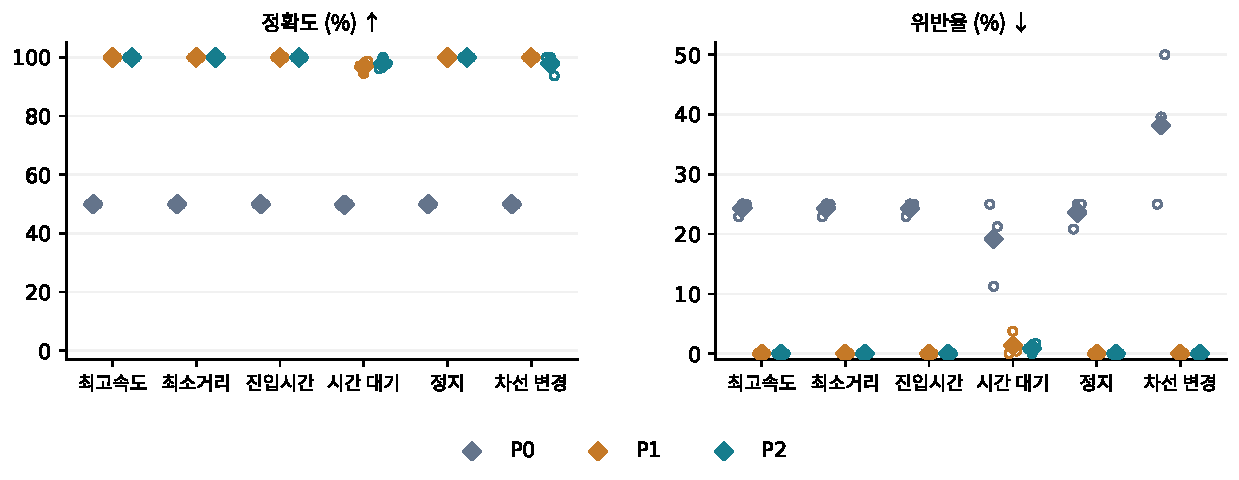
\includegraphics[width=\linewidth,height=.39\textheight,keepaspectratio]{figures/task-performance-ko.pdf}
\par\small\raggedright 그림 6. 정확도와 위반율의 과제별 비교. 큰 점은 평균, 작은 점은 세 시드 값이다. 선으로 과제 간 추세를 만들지 않았으며, 0\% 위반은 평가 표본에서 위반을 관측하지 않았다는 뜻이다.
\end{minipage}\par\smallskip

P2가 P1을 모든 시드·조건에서 능가하지는 않는다. 여기서는 P0 대비 두 경로의 관측 효과를 보고하며, P1–P2의 정형적 비열등성은 검정하지 않았다.\par

\section*{C. 제약 변경과 연결의 영향}

같은 장면의 제약만 바꾸는 계약쌍에서 P0의 정확도는 세 과제군 모두 0\%였다. 시간·정적·기동 과제군 순으로 P1은 93.61\%, 100\%, 100\%, P2는 96.11\%, 100\%, 97.92\%였다. 이는 제약을 제공받은 모델이 같은 시각 입력에서도 계약에 따라 선택을 달리할 수 있음을 보여준다. P0의 낮은 값은 계약 정보가 없는 과제 구성과 함께 해석해야 한다.\par

학습 시 사례와 제약의 대응을 뒤섞고 평가에서는 정상 제약을 제공하는 대조 조건의 정확도는 시간 50.56\%, 정적 50.69\%, 기동 49.65\%였다. 시간 과제는 자연어 제약을, 새 정적·기동 과제는 같은 유형 내 P2 CNL을 교란했으므로 동일한 교란 구현의 통합 추정치로 합치지 않는다. 결과는 문장 추가 자체보다 올바른 사례–제약 연결의 중요성을 지지한다.\par

\par\smallskip\noindent\begin{minipage}{\linewidth}\centering
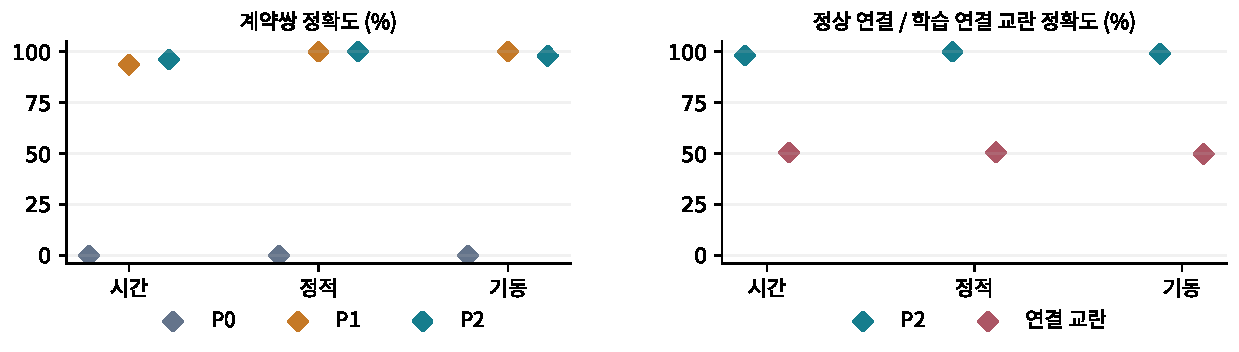
\includegraphics[width=\linewidth,height=.39\textheight,keepaspectratio]{figures/contract-linkage-ko.pdf}
\par\small\raggedright 그림 7. 왼쪽은 두 계약을 모두 맞힌 비율, 오른쪽은 정상 연결의 P2와 학습 연결 교란 조건의 행동 정확도이다. 점은 세 시드 평균이다. 정적·기동은 각각 하위 유형을 합친 과제군 결과이다.
\end{minipage}\par\smallskip

실제 예측의 한 사례에서 해소 11.0초·대기 1.5초일 때 P0는 11.5초 진입, P1·P2는 허용 경계인 12.5초 진입을 선택했다. P2가 다른 사례의 경계보다 0.1초 일찍 진입한 잔여 위반도 있었다. 사후 선택한 두 설명 사례의 상세는 부가자료 S5에 제시한다.\par

\newpage
\section*{D. 명세와 CNL의 검사 가능성}

스키마·근거·Core 판정·CNL 대응의 검사 경로에 부정 의미, 임계값, 해제 조건, 비교 연산, 단위 관련 오류를 주입했다. 여섯 유형 각 24건의 상세 결과와 검사 층은 부가자료 S3에 제시한다. 이 품질 평가는 모델 정확도와 별개이다.\par

\par\smallskip\noindent\begin{minipage}{\linewidth}
\textbf{표 E3. 명세·CNL 검사 결과}\par

\par\smallskip\noindent\begin{minipage}{\linewidth}\small
\begin{tabular}{@{}>{\raggedright\arraybackslash}p{\dimexpr 0.2300\linewidth-3.680pt\relax}>{\raggedright\arraybackslash}p{\dimexpr 0.3000\linewidth-4.800pt\relax}>{\raggedright\arraybackslash}p{\dimexpr 0.4700\linewidth-7.520pt\relax}@{}}
\toprule
\textbf{입력 유형} & \textbf{건수} & \textbf{검사 결과} \\
\midrule
지원 오류 6종 & 144 & 144 탐지, 미탐 0 \\
근거와 명세의 공유 오류 & 24 & 탐지 0, 미탐 24 \\
정상 계약 & 24 & 24 수용, 오탐 0 \\
\bottomrule\end{tabular}\end{minipage}\par\smallskip
\end{minipage}\par\smallskip

전체 오류 168건의 탐지율은 85.71\%였다. 이는 SAT 풀이만의 성과가 아니라 여러 검사 층의 결과이며, 신뢰한 근거와 명세가 함께 틀리면 오류가 남을 수 있다. 따라서 만족 가능성과 근거의 사실성은 구분한다.\par

시간 경계 질의 100건은 SAT 76건·UNSAT 24건으로 모두 예상과 일치했고 UNKNOWN은 없었다. 추가 과제의 후보 검사와 모델 예측 판정 대조는 부가자료 S8에 제시한다.\par

\par\smallskip\noindent\begin{minipage}{\linewidth}\centering
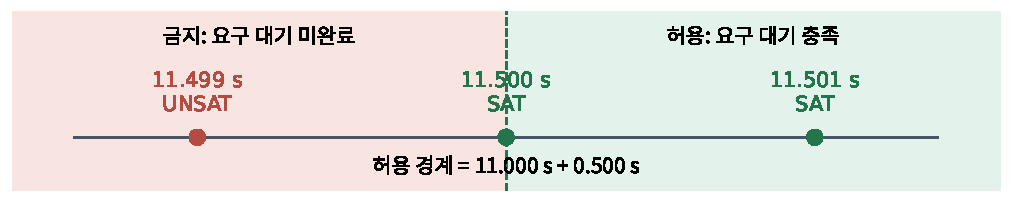
\includegraphics[width=\linewidth,height=.39\textheight,keepaspectratio]{figures/smt-boundary-ko.pdf}
\par\small\raggedright 그림 8. 11.000초 해소 후 0.500초 대기하는 계약의 경계 질의. 11.499초 진입은 UNSAT, 11.500초와 11.501초는 SAT이다. 그림은 경계 주변 1ms 간격을 확대한 논리 시간축이며 실제 차량 제어 정밀도를 뜻하지 않는다.
\end{minipage}\par\smallskip

여기서 UNSAT는 잘못된 명세 수가 아니라 계약과 금지 행동의 양립 불가능성을 뜻한다. 반대로 오류 주입으로 대기를 100ms 늘리면 원래 허용할 질의가 UNSAT가 되고, 해제 조건을 삭제하면 금지할 질의가 SAT가 된다. 기대와 다른 판정은 원 근거·임계값·조항을 점검하고 수정 후 양쪽 경계를 재검증해야 한다. 기본 계약 자체가 UNSAT이거나 UNKNOWN이면 승인 근거로 사용하지 않는다. 대표 충돌 집합과 상세 처리 사례는 부가자료에 보존한다.\par

\section*{E. 미학습 조건과 해석 범위}

\par\smallskip\noindent\begin{minipage}{\linewidth}
\textbf{표 E4. 미학습 수치·시간의 정확도 / 위반율. 단위 \%, 세 시드 평균}\par

\par\smallskip\noindent\begin{minipage}{\linewidth}\small
\begin{tabular}{@{}>{\raggedright\arraybackslash}p{\dimexpr 0.2800\linewidth-6.720pt\relax}>{\raggedright\arraybackslash}p{\dimexpr 0.2400\linewidth-5.760pt\relax}>{\raggedright\arraybackslash}p{\dimexpr 0.2400\linewidth-5.760pt\relax}>{\raggedright\arraybackslash}p{\dimexpr 0.2400\linewidth-5.760pt\relax}@{}}
\toprule
\textbf{과제군} & \textbf{P0} & \textbf{P1} & \textbf{P2} \\
\midrule
시간 & 49.86 / 18.47 & 96.67 / 2.22 & 96.67 / 1.53 \\
정적 & 50.00 / 22.92 & 99.54 / 0.00 & 97.22 / 0.23 \\
기동 & 50.00 / 30.90 & 100.00 / 0.00 & 98.96 / 0.00 \\
\bottomrule\end{tabular}\end{minipage}\par\smallskip
\end{minipage}\par\smallskip

학습하지 않은 수치·시간에서도 두 제약 강화 경로는 P0보다 높은 성능을 보였다. 다만 새로운 표현을 수용하는 정도는 과제별로 달랐다. 예를 들어 정적 표현 변경에서 P2 정확도는 80.32\%, 위반율은 7.87\%였다. 표현 변경·복합 조건·이미지 개입과 명세 기반 비용 추가 학습은 지원 경로의 보조 진단으로 분리하여, 유리한 결과와 불리한 결과 모두 부가자료에 보고한다.\par

본 결과는 공급된 합성 제약과 유한 후보에서의 효과이다. 텍스트 수치·반복 그림·단일 모델·세 시드에 한정되므로 실제 도로의 시각 이해, 폐루프 안전성이나 Alpamayo 학습으로 확대하지 않는다. 제약 제공 효과와 검증 자체의 인과 효과를 구분하며, 상세 변동·조건부 구간·기존 운영 기준의 판정은 부가자료에 보존한다.\par

종합하면, 여러 행동 과제에서 CoC 제약 강화의 효과가 관찰되었으며, EBLC 기반 지원 경로는 높은 행동 선택 성능과 함께 제약의 오류 및 허용·금지 경계를 검사하는 수단을 제공하였다.\par

부가자료: \href{\detokenize{ieee-access-experiments-supplement-v01-ko.pdf}}{상세 실험 결과 및 재현 근거}.\par
\end{document}